\documentclass{standalone}
\usepackage[margin=1in]{geometry}
\usepackage[hang,small,bf]{caption}
\usepackage{tikz}
\usepackage{braket}
\usetikzlibrary{backgrounds,shadows.blur,fit,decorations.pathreplacing,shapes}

\begin{document}
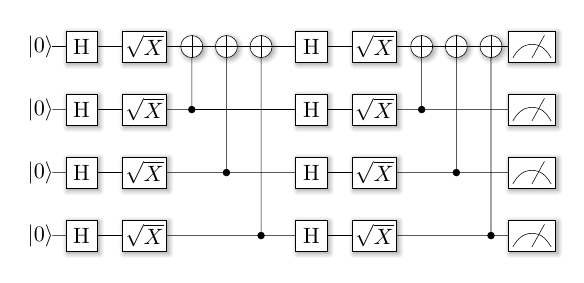
\begin{tikzpicture}[scale=0.8, transform shape]

\tikzstyle{basicshadow}=[blur shadow={shadow blur steps=8, shadow xshift=0.7pt, shadow yshift=-0.7pt, shadow scale=1.02}]\tikzstyle{basic}=[draw,fill=white,basicshadow]
\tikzstyle{operator}=[basic,minimum size=1.5em]
\tikzstyle{phase}=[fill=black,shape=circle,minimum size=0.1cm,inner sep=0pt,outer sep=0pt,draw=black]
\tikzstyle{none}=[inner sep=0pt,outer sep=-.5pt,minimum height=0.5cm+1pt]
\tikzstyle{measure}=[operator,inner sep=0pt,minimum height=0.5cm, minimum width=0.75cm]
\tikzstyle{xstyle}=[circle,basic,minimum height=0.35cm,minimum width=0.35cm,inner sep=-1pt,very thin]
\tikzset{
shadowed/.style={preaction={transform canvas={shift={(0.5pt,-0.5pt)}}, draw=gray, opacity=0.4}},
}
\tikzstyle{swapstyle}=[inner sep=-1pt, outer sep=-1pt, minimum width=0pt]
\tikzstyle{edgestyle}=[very thin]

\node[none] (line0_gate0) at (0.1,-0) {$\Ket{0}$};
\node[none] (line0_gate1) at (0.5,-0) {};
\node[none,minimum height=0.5cm,outer sep=0] (line0_gate2) at (0.75,-0) {};
\node[none] (line0_gate3) at (1.0,-0) {};
\draw[operator,edgestyle,outer sep=0.5cm] ([yshift=0.25cm]line0_gate1) rectangle ([yshift=-0.25cm]line0_gate3) node[pos=.5] {H};
\draw (line0_gate0) edge[edgestyle] (line0_gate1);
\node[none] (line0_gate4) at (1.4000000000000001,-0) {};
\node[none,minimum height=0.5cm,outer sep=0] (line0_gate5) at (1.75,-0) {};
\node[none] (line0_gate6) at (2.1,-0) {};
\draw[operator,edgestyle,outer sep=0.7cm] ([yshift=0.25cm]line0_gate4) rectangle ([yshift=-0.25cm]line0_gate6) node[pos=.5] {$\sqrt{X}$};
\draw (line0_gate3) edge[edgestyle] (line0_gate4);
\node[none] (line1_gate0) at (0.1,-1) {$\Ket{0}$};
\node[none] (line1_gate1) at (0.5,-1) {};
\node[none,minimum height=0.5cm,outer sep=0] (line1_gate2) at (0.75,-1) {};
\node[none] (line1_gate3) at (1.0,-1) {};
\draw[operator,edgestyle,outer sep=0.5cm] ([yshift=0.25cm]line1_gate1) rectangle ([yshift=-0.25cm]line1_gate3) node[pos=.5] {H};
\draw (line1_gate0) edge[edgestyle] (line1_gate1);
\node[none] (line1_gate4) at (1.4000000000000001,-1) {};
\node[none,minimum height=0.5cm,outer sep=0] (line1_gate5) at (1.75,-1) {};
\node[none] (line1_gate6) at (2.1,-1) {};
\draw[operator,edgestyle,outer sep=0.7cm] ([yshift=0.25cm]line1_gate4) rectangle ([yshift=-0.25cm]line1_gate6) node[pos=.5] {$\sqrt{X}$};
\draw (line1_gate3) edge[edgestyle] (line1_gate4);
\node[xstyle] (line0_gate7) at (2.5000000000000004,-0) {};
\draw[edgestyle] (line0_gate7.north)--(line0_gate7.south);
\draw[edgestyle] (line0_gate7.west)--(line0_gate7.east);
\node[phase] (line1_gate7) at (2.5000000000000004,-1) {};
\draw (line1_gate7) edge[edgestyle] (line0_gate7);
\draw (line0_gate6) edge[edgestyle] (line0_gate7);
\draw (line1_gate6) edge[edgestyle] (line1_gate7);
\node[none] (line2_gate0) at (0.1,-2) {$\Ket{0}$};
\node[none] (line2_gate1) at (0.5,-2) {};
\node[none,minimum height=0.5cm,outer sep=0] (line2_gate2) at (0.75,-2) {};
\node[none] (line2_gate3) at (1.0,-2) {};
\draw[operator,edgestyle,outer sep=0.5cm] ([yshift=0.25cm]line2_gate1) rectangle ([yshift=-0.25cm]line2_gate3) node[pos=.5] {H};
\draw (line2_gate0) edge[edgestyle] (line2_gate1);
\node[none] (line2_gate4) at (1.4000000000000001,-2) {};
\node[none,minimum height=0.5cm,outer sep=0] (line2_gate5) at (1.75,-2) {};
\node[none] (line2_gate6) at (2.1,-2) {};
\draw[operator,edgestyle,outer sep=0.7cm] ([yshift=0.25cm]line2_gate4) rectangle ([yshift=-0.25cm]line2_gate6) node[pos=.5] {$\sqrt{X}$};
\draw (line2_gate3) edge[edgestyle] (line2_gate4);
\node[xstyle] (line0_gate8) at (3.0500000000000007,-0) {};
\draw[edgestyle] (line0_gate8.north)--(line0_gate8.south);
\draw[edgestyle] (line0_gate8.west)--(line0_gate8.east);
\node[phase] (line2_gate7) at (3.0500000000000007,-2) {};
\draw (line2_gate7) edge[edgestyle] (line0_gate8);
\draw (line0_gate7) edge[edgestyle] (line0_gate8);
\draw (line2_gate6) edge[edgestyle] (line2_gate7);
\node[none] (line3_gate0) at (0.1,-3) {$\Ket{0}$};
\node[none] (line3_gate1) at (0.5,-3) {};
\node[none,minimum height=0.5cm,outer sep=0] (line3_gate2) at (0.75,-3) {};
\node[none] (line3_gate3) at (1.0,-3) {};
\draw[operator,edgestyle,outer sep=0.5cm] ([yshift=0.25cm]line3_gate1) rectangle ([yshift=-0.25cm]line3_gate3) node[pos=.5] {H};
\draw (line3_gate0) edge[edgestyle] (line3_gate1);
\node[none] (line3_gate4) at (1.4000000000000001,-3) {};
\node[none,minimum height=0.5cm,outer sep=0] (line3_gate5) at (1.75,-3) {};
\node[none] (line3_gate6) at (2.1,-3) {};
\draw[operator,edgestyle,outer sep=0.7cm] ([yshift=0.25cm]line3_gate4) rectangle ([yshift=-0.25cm]line3_gate6) node[pos=.5] {$\sqrt{X}$};
\draw (line3_gate3) edge[edgestyle] (line3_gate4);
\node[xstyle] (line0_gate9) at (3.600000000000001,-0) {};
\draw[edgestyle] (line0_gate9.north)--(line0_gate9.south);
\draw[edgestyle] (line0_gate9.west)--(line0_gate9.east);
\node[phase] (line3_gate7) at (3.600000000000001,-3) {};
\draw (line3_gate7) edge[edgestyle] (line0_gate9);
\draw (line0_gate8) edge[edgestyle] (line0_gate9);
\draw (line3_gate6) edge[edgestyle] (line3_gate7);
\node[none] (line0_gate10) at (4.15,-0) {};
\node[none,minimum height=0.5cm,outer sep=0] (line0_gate11) at (4.4,-0) {};
\node[none] (line0_gate12) at (4.65,-0) {};
\draw[operator,edgestyle,outer sep=0.5cm] ([yshift=0.25cm]line0_gate10) rectangle ([yshift=-0.25cm]line0_gate12) node[pos=.5] {H};
\draw (line0_gate9) edge[edgestyle] (line0_gate10);
\node[none] (line0_gate13) at (5.05,-0) {};
\node[none,minimum height=0.5cm,outer sep=0] (line0_gate14) at (5.3999999999999995,-0) {};
\node[none] (line0_gate15) at (5.75,-0) {};
\draw[operator,edgestyle,outer sep=0.7cm] ([yshift=0.25cm]line0_gate13) rectangle ([yshift=-0.25cm]line0_gate15) node[pos=.5] {$\sqrt{X}$};
\draw (line0_gate12) edge[edgestyle] (line0_gate13);
\node[none] (line1_gate8) at (4.15,-1) {};
\node[none,minimum height=0.5cm,outer sep=0] (line1_gate9) at (4.4,-1) {};
\node[none] (line1_gate10) at (4.65,-1) {};
\draw[operator,edgestyle,outer sep=0.5cm] ([yshift=0.25cm]line1_gate8) rectangle ([yshift=-0.25cm]line1_gate10) node[pos=.5] {H};
\draw (line1_gate7) edge[edgestyle] (line1_gate8);
\node[none] (line1_gate11) at (5.05,-1) {};
\node[none,minimum height=0.5cm,outer sep=0] (line1_gate12) at (5.3999999999999995,-1) {};
\node[none] (line1_gate13) at (5.75,-1) {};
\draw[operator,edgestyle,outer sep=0.7cm] ([yshift=0.25cm]line1_gate11) rectangle ([yshift=-0.25cm]line1_gate13) node[pos=.5] {$\sqrt{X}$};
\draw (line1_gate10) edge[edgestyle] (line1_gate11);
\node[xstyle] (line0_gate16) at (6.1499999999999995,-0) {};
\draw[edgestyle] (line0_gate16.north)--(line0_gate16.south);
\draw[edgestyle] (line0_gate16.west)--(line0_gate16.east);
\node[phase] (line1_gate14) at (6.1499999999999995,-1) {};
\draw (line1_gate14) edge[edgestyle] (line0_gate16);
\draw (line0_gate15) edge[edgestyle] (line0_gate16);
\draw (line1_gate13) edge[edgestyle] (line1_gate14);
\node[none] (line2_gate8) at (4.15,-2) {};
\node[none,minimum height=0.5cm,outer sep=0] (line2_gate9) at (4.4,-2) {};
\node[none] (line2_gate10) at (4.65,-2) {};
\draw[operator,edgestyle,outer sep=0.5cm] ([yshift=0.25cm]line2_gate8) rectangle ([yshift=-0.25cm]line2_gate10) node[pos=.5] {H};
\draw (line2_gate7) edge[edgestyle] (line2_gate8);
\node[none] (line2_gate11) at (5.05,-2) {};
\node[none,minimum height=0.5cm,outer sep=0] (line2_gate12) at (5.3999999999999995,-2) {};
\node[none] (line2_gate13) at (5.75,-2) {};
\draw[operator,edgestyle,outer sep=0.7cm] ([yshift=0.25cm]line2_gate11) rectangle ([yshift=-0.25cm]line2_gate13) node[pos=.5] {$\sqrt{X}$};
\draw (line2_gate10) edge[edgestyle] (line2_gate11);
\node[xstyle] (line0_gate17) at (6.699999999999998,-0) {};
\draw[edgestyle] (line0_gate17.north)--(line0_gate17.south);
\draw[edgestyle] (line0_gate17.west)--(line0_gate17.east);
\node[phase] (line2_gate14) at (6.699999999999998,-2) {};
\draw (line2_gate14) edge[edgestyle] (line0_gate17);
\draw (line0_gate16) edge[edgestyle] (line0_gate17);
\draw (line2_gate13) edge[edgestyle] (line2_gate14);
\node[none] (line3_gate8) at (4.15,-3) {};
\node[none,minimum height=0.5cm,outer sep=0] (line3_gate9) at (4.4,-3) {};
\node[none] (line3_gate10) at (4.65,-3) {};
\draw[operator,edgestyle,outer sep=0.5cm] ([yshift=0.25cm]line3_gate8) rectangle ([yshift=-0.25cm]line3_gate10) node[pos=.5] {H};
\draw (line3_gate7) edge[edgestyle] (line3_gate8);
\node[none] (line3_gate11) at (5.05,-3) {};
\node[none,minimum height=0.5cm,outer sep=0] (line3_gate12) at (5.3999999999999995,-3) {};
\node[none] (line3_gate13) at (5.75,-3) {};
\draw[operator,edgestyle,outer sep=0.7cm] ([yshift=0.25cm]line3_gate11) rectangle ([yshift=-0.25cm]line3_gate13) node[pos=.5] {$\sqrt{X}$};
\draw (line3_gate10) edge[edgestyle] (line3_gate11);
\node[xstyle] (line0_gate18) at (7.249999999999997,-0) {};
\draw[edgestyle] (line0_gate18.north)--(line0_gate18.south);
\draw[edgestyle] (line0_gate18.west)--(line0_gate18.east);
\node[phase] (line3_gate14) at (7.249999999999997,-3) {};
\draw (line3_gate14) edge[edgestyle] (line0_gate18);
\draw (line0_gate17) edge[edgestyle] (line0_gate18);
\draw (line3_gate13) edge[edgestyle] (line3_gate14);
\node[measure,edgestyle] (line0_gate19) at (7.899999999999997,-0) {};
\draw[edgestyle] ([yshift=-0.18cm,xshift=0.07500000000000001cm]line0_gate19.west) to [out=60,in=180] ([yshift=0.035cm]line0_gate19.center) to [out=0, in=120] ([yshift=-0.18cm,xshift=-0.07500000000000001cm]line0_gate19.east);
\draw[edgestyle] ([yshift=-0.18cm]line0_gate19.center) to ([yshift=-0.07500000000000001cm,xshift=-0.18cm]line0_gate19.north east);
\draw (line0_gate18) edge[edgestyle] (line0_gate19);
\node[measure,edgestyle] (line1_gate15) at (7.899999999999997,-1) {};
\draw[edgestyle] ([yshift=-0.18cm,xshift=0.07500000000000001cm]line1_gate15.west) to [out=60,in=180] ([yshift=0.035cm]line1_gate15.center) to [out=0, in=120] ([yshift=-0.18cm,xshift=-0.07500000000000001cm]line1_gate15.east);
\draw[edgestyle] ([yshift=-0.18cm]line1_gate15.center) to ([yshift=-0.07500000000000001cm,xshift=-0.18cm]line1_gate15.north east);
\draw (line1_gate14) edge[edgestyle] (line1_gate15);
\node[measure,edgestyle] (line2_gate15) at (7.899999999999997,-2) {};
\draw[edgestyle] ([yshift=-0.18cm,xshift=0.07500000000000001cm]line2_gate15.west) to [out=60,in=180] ([yshift=0.035cm]line2_gate15.center) to [out=0, in=120] ([yshift=-0.18cm,xshift=-0.07500000000000001cm]line2_gate15.east);
\draw[edgestyle] ([yshift=-0.18cm]line2_gate15.center) to ([yshift=-0.07500000000000001cm,xshift=-0.18cm]line2_gate15.north east);
\draw (line2_gate14) edge[edgestyle] (line2_gate15);
\node[measure,edgestyle] (line3_gate15) at (7.899999999999997,-3) {};
\draw[edgestyle] ([yshift=-0.18cm,xshift=0.07500000000000001cm]line3_gate15.west) to [out=60,in=180] ([yshift=0.035cm]line3_gate15.center) to [out=0, in=120] ([yshift=-0.18cm,xshift=-0.07500000000000001cm]line3_gate15.east);
\draw[edgestyle] ([yshift=-0.18cm]line3_gate15.center) to ([yshift=-0.07500000000000001cm,xshift=-0.18cm]line3_gate15.north east);
\draw (line3_gate14) edge[edgestyle] (line3_gate15);

\end{tikzpicture}
\end{document}
